% Options for packages loaded elsewhere
\PassOptionsToPackage{unicode}{hyperref}
\PassOptionsToPackage{hyphens}{url}
%
\documentclass[
]{book}
\usepackage{amsmath,amssymb}
\usepackage{iftex}
\ifPDFTeX
  \usepackage[T1]{fontenc}
  \usepackage[utf8]{inputenc}
  \usepackage{textcomp} % provide euro and other symbols
\else % if luatex or xetex
  \usepackage{unicode-math} % this also loads fontspec
  \defaultfontfeatures{Scale=MatchLowercase}
  \defaultfontfeatures[\rmfamily]{Ligatures=TeX,Scale=1}
\fi
\usepackage{lmodern}
\ifPDFTeX\else
  % xetex/luatex font selection
\fi
% Use upquote if available, for straight quotes in verbatim environments
\IfFileExists{upquote.sty}{\usepackage{upquote}}{}
\IfFileExists{microtype.sty}{% use microtype if available
  \usepackage[]{microtype}
  \UseMicrotypeSet[protrusion]{basicmath} % disable protrusion for tt fonts
}{}
\makeatletter
\@ifundefined{KOMAClassName}{% if non-KOMA class
  \IfFileExists{parskip.sty}{%
    \usepackage{parskip}
  }{% else
    \setlength{\parindent}{0pt}
    \setlength{\parskip}{6pt plus 2pt minus 1pt}}
}{% if KOMA class
  \KOMAoptions{parskip=half}}
\makeatother
\usepackage{xcolor}
\usepackage{longtable,booktabs,array}
\usepackage{calc} % for calculating minipage widths
% Correct order of tables after \paragraph or \subparagraph
\usepackage{etoolbox}
\makeatletter
\patchcmd\longtable{\par}{\if@noskipsec\mbox{}\fi\par}{}{}
\makeatother
% Allow footnotes in longtable head/foot
\IfFileExists{footnotehyper.sty}{\usepackage{footnotehyper}}{\usepackage{footnote}}
\makesavenoteenv{longtable}
\usepackage{graphicx}
\makeatletter
\def\maxwidth{\ifdim\Gin@nat@width>\linewidth\linewidth\else\Gin@nat@width\fi}
\def\maxheight{\ifdim\Gin@nat@height>\textheight\textheight\else\Gin@nat@height\fi}
\makeatother
% Scale images if necessary, so that they will not overflow the page
% margins by default, and it is still possible to overwrite the defaults
% using explicit options in \includegraphics[width, height, ...]{}
\setkeys{Gin}{width=\maxwidth,height=\maxheight,keepaspectratio}
% Set default figure placement to htbp
\makeatletter
\def\fps@figure{htbp}
\makeatother
\setlength{\emergencystretch}{3em} % prevent overfull lines
\providecommand{\tightlist}{%
  \setlength{\itemsep}{0pt}\setlength{\parskip}{0pt}}
\setcounter{secnumdepth}{5}
\usepackage{booktabs}
\usepackage[ngerman,provide=*]{babel}
\usepackage{amsthm}
\makeatletter
\def\thm@space@setup{%
  \thm@preskip=8pt plus 2pt minus 4pt
  \thm@postskip=\thm@preskip
}
\makeatother

% Redefine names for various elements
\renewcommand{\figurename}{Abbildung}
\renewcommand{\tablename}{Tabelle}
\renewcommand{\contentsname}{Inhaltsverzeichnis}
\renewcommand{\partname}{Teil}
\renewcommand{\chaptername}{Kapitel}
\renewcommand{\appendixname}{Anhang}

% The \equationname is not a standard LaTeX command, so we'll define it
\newcommand{\equationname}{Gleichung}

% Redefine proof name
\renewcommand{\proofname}{Beweis}

% Ensure German captions are used
\addto\captionsgerman{
  \renewcommand{\partname}{Teil}
  \renewcommand{\chaptername}{Kapitel}
}

\usepackage{tcolorbox}
\usepackage{xcolor}



\newenvironment{caution}{
  \begin{itemize}
  \renewcommand{\labelitemi}{
    \raisebox{-.7\height}[0pt][0pt]{
      {\setkeys{Gin}{width=3em,keepaspectratio}
        
\includegraphics{figures/icons/caution.png}}
    }
  }
  \setlength{\fboxsep}{1em}
  \begin{tcolorbox}[
  colback=gray!10,
    colframe=gray!50,
    title=\textbf{Achtung},
    fonttitle=\bfseries,
    coltitle=black,
    colbacktitle=yellow!50,
    sharp corners=south] % Optional: Use tcolorbox for better visuals
  \item
  }
  {
  \end{tcolorbox}
  \end{itemize}
  }{}

\usepackage{amsthm}
\ifLuaTeX
  \usepackage{selnolig}  % disable illegal ligatures
\fi
\usepackage[]{natbib}
\bibliographystyle{apalike}
\usepackage{bookmark}
\IfFileExists{xurl.sty}{\usepackage{xurl}}{} % add URL line breaks if available
\urlstyle{same}
\hypersetup{
  pdftitle={Statistik 1},
  pdfauthor={Daniel J. F. Gerber},
  hidelinks,
  pdfcreator={LaTeX via pandoc}}

\title{Statistik 1}
\author{Daniel J. F. Gerber}
\date{2024-10-05}

\usepackage{amsthm}
\newtheorem{theorem}{Theorem}[chapter]
\newtheorem{lemma}{Lemma}[chapter]
\newtheorem{corollary}{Corollary}[chapter]
\newtheorem{proposition}{Proposition}[chapter]
\newtheorem{conjecture}{Conjecture}[chapter]
\theoremstyle{definition}
\newtheorem{definition}{Definition}[chapter]
\theoremstyle{definition}
\newtheorem{example}{Beispiel}[chapter]
\theoremstyle{definition}
\newtheorem{exercise}{Übung}[chapter]
\theoremstyle{definition}
\newtheorem{hypothesis}{Hypothese}[chapter]
\theoremstyle{remark}
\newtheorem*{remark}{Hinweis}
\newtheorem*{solution}{Lösung}
\begin{document}
\maketitle

{
\setcounter{tocdepth}{1}
\tableofcontents
}
\chapter*{Vorwort}\label{vorwort}
\addcontentsline{toc}{chapter}{Vorwort}

Dieses Buch ist im Rahmen meiner Lehrtätigkeit an der FHNW entstanden und frei verfügbar.

\chapter{Einleitung}\label{einleitung}

\section{Worum geht es?}\label{worum-geht-es}

\section{Inhaltlicher Aufbau}\label{inhaltlicher-aufbau}

Dieses Buch umfasst die untenstehenden Inhalte. Die Inhalte wurden hier nach Zwecken sortiert angeordnet:

Stichprobe beschreiben (\textbf{deskriptive Statistik}):

\begin{itemize}
\tightlist
\item
  Arithmetisches Mittel
\item
  Median
\item
  Quantile
\item
  Anteil
\item
  Odds Ratio
\item
  Relatives Risiko
\end{itemize}

Population beschreiben (\textbf{Wahrscheinlichkeitslehre}):

\begin{itemize}
\tightlist
\item
  Zufallsvariable
\item
  Erwartungswert
\item
  Standardabweichung
\item
  Varianz
\item
  Wahrscheinlichkeitsdichte
\item
  Wahrscheinlichkeitsverteilung
\item
  Verteilungen
\end{itemize}

Populationsparameter aus Stichproben schätzen (\textbf{Konfidenzintervalle} + Stichprobengrösse):

\begin{itemize}
\tightlist
\item
  Mittelwert
\item
  Standardabweichung
\item
  Anteil
\item
  Berichten
\item
  Darstellen
\end{itemize}

Aussagen auf die Population aufgrund von Stichproben machen (Test-Theorie):

\begin{itemize}
\tightlist
\item
  Effektstärke
\item
  Berichten
\item
  T-Test (1 Stichprobe)
\item
  T-Test (2 Stichproben), Welch-Test
\item
  Welch Test
\item
  U-Test
\item
  Korrelation absichern gegen 0
\item
  Vierfelder/Mehrfeldertest
\end{itemize}

Zusammenhänge beschreiben (Zusammenhangsmasse):

\begin{itemize}
\tightlist
\item
  Pearsons r
\item
  Spearmans rho
\item
  Vierfelderkorrelation / Phi
\item
  Punktbiseriale Korrelation
\item
  Kontingenzkoeffizient
\item
  Cramérs V
\end{itemize}

Die Inhalte nach Zweck zu gruppieren ist eine Option, die andere ist die Verfahren der Skalierung der Variablen folgend aufzubauen. Bei dieser Gruppierung ist der Zweck nicht direkt ersichtlich, dafür ist einfacher zu begreiffen welches Verfahren für welche Ausgangslage geeignet ist. Diese Gruppierung wurde für die präsentation der Inhalte in diesem Buch gewählt.

\section{Wie soll ich dieses Buch lesen?}\label{wie-soll-ich-dieses-buch-lesen}

Dieses Buch enthält zu jedem Thema eine kurze Beschreibung der Theorie, Beispiele und Übungen. Das selbstständige Lösen der Übungen ist unerlässlich für das Verständnis und die emanzipation im korrekten Umgang mit Daten. Ohne Übungen fehlt die Auseinandersetzung mit dem Unterrichtsstoff und ohne diese fällt es den allermeisten schwer sogar einfachste Zusammenhänge zu begreiffen. Es wird deshalb empfohlen, dass die Übungen zum jeweiligen Thema zeitnah zur Theorie gelöst werden. Damit überprüft werden kann, ob die Übungen richtig gelöst wurden, ist zu jeder Übung eine kurze Lösung hinterlegt. Wer beim ersten selbstständigen Versuch der Übungslösung scheitert - was garantiert den meisten Lesenden hier ein oder mehrmals passieren wird -, kann die Übung mit Hilfe der Lösung lösen und zu einem späteren Zeitpunkt die Übung selbstständig nochmal machen ohne Lösung. Für die Statistik ist es also \textbf{nicht} genug den Stoff einmal auswendig zu lernen, übung ist unerlässlich.

\section{Formeln}\label{formeln}

Die Statistik bedient sich der universellen Sprache der Formeln. Es ist deshalb unerlässlich einige Formeln zu verstehen. Das Verständnis von Formeln ist für ungeübte Lesende verwirrend und schwierig. Deshalb wird dieses Verständnis in diesem Buch nach und nach aufgebaut. Dazu werden Teilformeln isoliert und erklärt und die Einflüsse der verschiedenen Kenngrössen in der Formel exploriert.

\section{Software}\label{software}

Für die Lösung der Übungen wird oft die freie Software Jamovi verwendet. Dem Leser wird deshalb empfohlen diese Software zu installieren. Für die Erstellung dieses Buches wurden ferner die folgenden Softwareprodukte verwendet:

\begin{itemize}
\tightlist
\item
  Jamovi software (Version 2.3.21.0)
\item
  Jamovi R-package \citep{R-jmv}
\item
  R \citep{R-base}
\item
  Tidyverse \citep{tidyverse2019}
\item
  Bookdown \citep{bookdown2016}
\end{itemize}

\part{Eine intervallskaliertes Merkmal}\label{part-eine-intervallskaliertes-merkmal}

\chapter{Intervallskalierte Merkmale}\label{intervallskalierte-merkmale}

\section{Was ist ein intervallskaliertes Merkmal?}\label{was-ist-ein-intervallskaliertes-merkmal}

Ein Merkmal ist dann intervallskaliert, wenn die einzelnen Beobachtungen in eine natürliche Reihenfolge gebracht werden können und zwischen dem tiefsten und höchsten möglichen Wert, alle erdenklichen Zwischenwerte möglich sind.

Ein Beispiel für ein intervallskaliertes Merkmal ist die Körpertemperatur. Beobachtungen der Körpertemperatur einer lebenden Person sind Werte zwischen ungefähr 10°C und 42°C. Es ist möglich zu sagen, dass eine Person mit 40°C Körpertemperatur eine höhere Temperatur hat als eine mit 38°C Körpertemperatur. Ausserdem sind alle erdenklichen Zwischenwerte möglich, so auch dass bei einer Person eine Körpertemperatur von 37.821239°C gemessen wird.

Ein weiteres Beispiel für ein intervallskaliertes Merkmal ist der Intelligenzquotient \emph{IQ}. Der IQ bewegt sich normalerweise zwischen 50 und 150, eine Person mit einem IQ von 105 hat einen höheren IQ als eine Person mit einem IQ von 103. Ausserdem sind IQ-Werte von 103.12 oder 118.9182 durchaus möglich.

Klicke hier, falls dir verhältnisskalierte Merkmale bekannt sind

Die folgende Diskussion ist auch auf verhältnisskalierte Merkmale anwendbar. Letztere sind intervallskalierte Merkmale, welche einen absoluten Nullpunkt aufweisen.

\section{Wie kann eine intervallskaliertes Merkmal beschrieben werden?}\label{wie-kann-eine-intervallskaliertes-merkmal-beschrieben-werden}

Eine Veterinärin möchte herausfinden, welche Körpertemperatur Enten aufweisen. Dazu untersucht sie 40 Enten und misst die Körpertemperaturen 42.01, 41.72, 41.51, 41.52, 41.5, 41.6, 41.46, 41.81, 42.14, 41.82, 42.06, 41.53, 41.66, 41.65, 41.46, 41.48, 41.92, 41.58, 41.32, 41.58, 41.81, 41.7, 41.62, 41.52, 41.89, 41.53, 41.67, 41.43, 42.18, 41.52, 41.82, 41.96, 41.8, 41.54, 41.88, 41.69, 41.92, 41.35, 41.07, 41.67.

Für einen Menschen ist es ziemlich schwierig direkt aus der Sichtung dieser Zahlen zu begreifen, welche Körpertemperatur Enten haben. Ein Mensch kann sich jedoch helfen, indem er die Zahlen zusammenfasst.

\subsection{Verteilung}\label{verteilung}

Um die Zahlen zusammenzufassen, kann die Veterinärin zum Beispiel Temperaturabschnitte von \(0.2\)°C betrachten und zählen wie viele Beobachtungen sie in den jeweiligen Abschnitten gemacht hat. Diese Zähldaten können tabellarisch oder grafisch mit einem Balkendiagramm dargestellt werden. Letzteres wird ein \textbf{Histogramm} genannt.

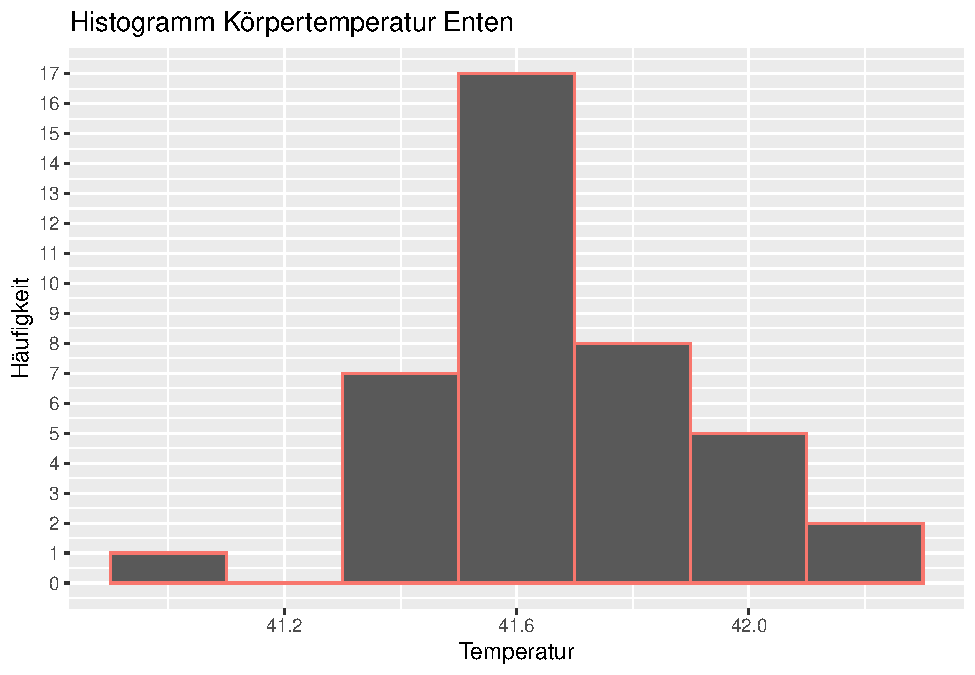
\includegraphics{aps_statistik1_files/figure-latex/enten_histogramm-1.pdf}

Aufgrund dieser Darstellung kann die Veterinärin nun sehen, wie häufig welche Körpertemperature sind. Dies wird die \textbf{Verteilung} des Merkmals genannt. Sie bemerkt zum Beispiel, dass Beobachtungen der Körpertemperatur rund um 41.6°C am häufigsten sind und tiefere und höhere Temperaturen seltener vorkommen. Auf einen Blick sieht sie auch, dass die Temperatur aller Enten zwischen 41°C und 42.2°C war.

Die Verteilung eines Merkmals zu kennen ist hilfreich, jedoch in vielen Situationen (z. B. in der Kommunikation) noch zu komplex. Einfacher ist es die Komplexität einer Verteilung auf zwei Faktoren herunterzubrechen: Die Zentralität und die Variabilität einse Merkmals.

\subsection{Zentralität}\label{zentralituxe4t}

Mit der Zentralität ist ein Wert gemeint, welcher die zentrale Tendenz des Merkmals abbildet. Um die Zentralität zu messen gibt es drei Möglichkeiten:

\begin{itemize}
\tightlist
\item
  Der \textbf{Modus} ist der am häufigsten vorkommende Wert. Im Beispiel ist das der Wert 41.52, welcher 3 mal und damit am häufigsten vorkommt.
\item
  Wenn die Werte des Merkmals aufsteigend sortiert werden und der Wert betrachtet wird, welcher die Beobachtungen in eine tiefere und eine höhere Hälfte teilt, dann wird dieser Wert als \textbf{Median} (abgekürtzt \emph{Mdn}, Symbol \(\tilde{x}\)) bezeichnet. Bei einer geraden Anzahl Beobachtungen, wird in der Regel der Durchschnittswert der beiden mittigsten Beobachtungen verwendet. Im Beispiel haben wir 40 Beobachtugen. Der Median entspricht also dem Durchschnittswert zwischen dem 20. und dem 21. der aufsteigend sortierten Werte 41.07, 41.32, 41.35, 41.43, 41.46, 41.46, 41.48, 41.5, 41.51, 41.52, 41.52, 41.52, 41.53, 41.53, 41.54, 41.58, 41.58, 41.6, 41.62, 41.65, 41.66, 41.67, 41.67, 41.69, 41.7, 41.72, 41.8, 41.81, 41.81, 41.82, 41.82, 41.88, 41.89, 41.92, 41.92, 41.96, 42.01, 42.06, 42.14, 42.18, also 41.655.
\item
  Das \textbf{arithmetische Mittel} (abgekürtzt \emph{M}, Symbol \(\bar{x}\)) bezeichnet, was gemeinhin mit Durchschnitt gemeint ist. Wenn wir die erste von insgesamt \(n\) Beobachtung mit \(x_1\) und die letzte Beobachtung mit \(x_n\) bezeichnen, so ist das aritmethische Mittel
\end{itemize}

\begin{equation}
\bar{x} = \frac{1}{n}\sum^n_{i=1} x_i
\label{eq:mean}
\end{equation}

Im Beispiel ist das arithmetische Mittel der Körpertemperaturen 41.6725.

\begin{caution}

\begin{remark}
\emph{Erklärung der Formel}: Hier wird zum ersten Mal eine Formel verwendet. \(\sum\) steht für die Summe von allen Beobachtungen \(x_i\), wenn der Index \(i\) in \(1\)-Schritten von der Zahl unter dem Summenzeichen \(i=1\) bis zu der Zahl oben am Summenzeichen \(i=n\) läuft. In unserem Beispiel ist \(n=40\), also ist \(i = 1, 2, 3, 4, \ldots, 39, 40\). Der Teil \(\sum^n_{i=1} x_i\) bedeutet also nichts anderes als \(x_1 + x_2 + \ldots + x_{39} + x_{40}\), also die Summe aller Beobachtungen. \(\frac{1}{n}\) bedeutet, dass wir diese Summe jetzt noch durch die Anzahl Beobachtungen teilen.

\emph{Welchen Einfluss haben die verschiedenen Einflussgrössen}: Dies wird in Übung \ref{exr:theorie-mdn-mean} erklärt.
\end{remark}

\end{caution}

Jedes dieser Masse für die Zentralität hat Vor- und Nachteile und sie werden dementsprechend in unterschiedlichen Situationen eingesetzt, siehe Übungen.

\subsection{Variabilität}\label{variabilituxe4t}

TODO: Quantile
TODO: Standardabweichung

\section{Übungen}\label{uxfcbungen}

\begin{exercise}
\protect\hypertarget{exr:enten-hist-mean-sd}{}\label{exr:enten-hist-mean-sd}\leavevmode

\begin{enumerate}
\def\labelenumi{(\alph{enumi})}
\tightlist
\item
  Versuch selbst ein Histogramm der Daten oben (\emph{Enten\_n40.sav}) mit Jamovi zu erstellen und begründe, weshalb es nicht gleich aussieht wie das Histogramm oben.
\item
  Berechne zusätzlich das arithmetische Mittel und die Standardabweichung des Merkmals.
\end{enumerate}

\end{exercise}

\begin{solution}
\leavevmode

\begin{figure}
  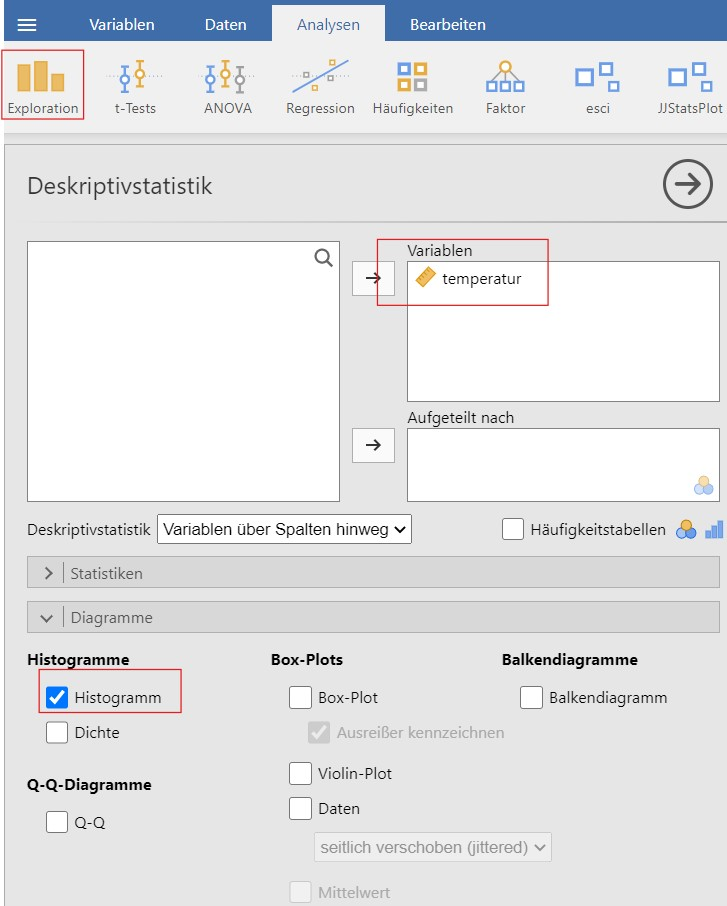
\includegraphics[width=0.5\linewidth]{figures/Enten_n40_instr_histogramm} 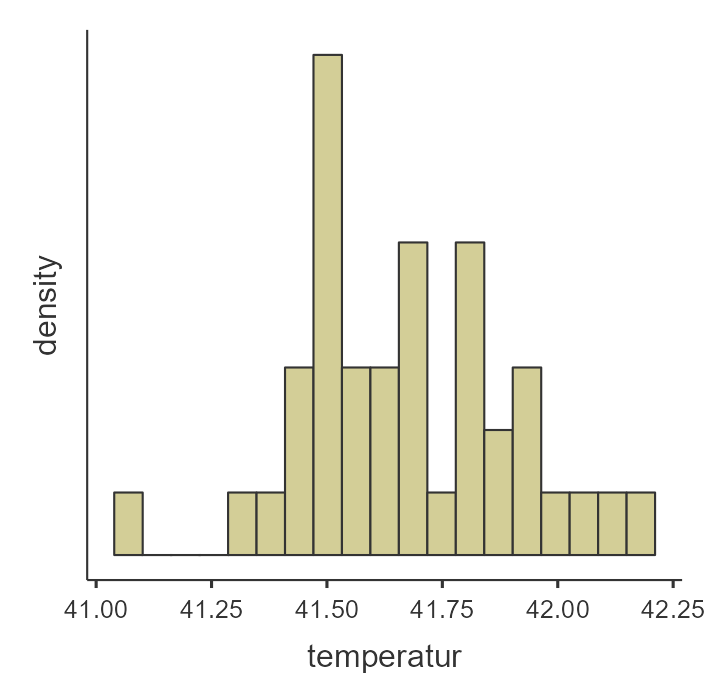
\includegraphics[width=0.5\linewidth]{figures/Enten_n40} \caption{Links: Jamovi-Anleitung zur Erstellung des Histogramms; rechts: Histogramm der Temperatur.}\label{fig:enten-hist-mean-sd}
  \end{figure}

\begin{enumerate}
\def\labelenumi{(\alph{enumi})}
\item
  Das Histogramm, siehe Abbildung \ref{fig:enten-hist-mean-sd} sieht nicht gleich aus, da Jamovi die Temperaturabschnitte kürzer gewählt hat nämlich bei 0.125°C statt 0.2°C wie oben im Text. In Jamovi gibt es aktuell keine Möglichkeit die Abschnittsweite anzupassen. Ein Histogramm sieht immer anders aus je nach ausgewählter Abschnittsweite.
\item
  TODO
\end{enumerate}

\end{solution}

\begin{exercise}
\protect\hypertarget{exr:theorie-mdn-mean}{}\label{exr:theorie-mdn-mean}

In einem psychologischen Test machen \(5\) Probandinnen die Werte \(18, 21, 20, 19, 22\). Um mit einer Zahl zu sagen, wo die Testresultate liegen wird ein zentraler Wert berechnet.

\begin{enumerate}
\def\labelenumi{(\alph{enumi})}
\tightlist
\item
  Wie gross ist das arithmetische Mittel und der Median dieser Werte?
\item
  Nehme an, der Testleiter hat den Wert der ersten Probandin falsch in seine Tabelle übertragen - statt \(18\) hat er \(81\) geschrieben. Wie gross ist das arithmetische Mittel und der Median dieser Werte in diesem Fall?
\item
  Was sagt dies über den Median und das arithmetische Mittel aus?
\end{enumerate}

\end{exercise}

\begin{solution}

Die Aufgabe kann im Kopf gelöst werden, oder mithilfe eines Taschenrechners, oder indem die Zahlen manuell bei Jamovi eingegeben werden.

\begin{enumerate}
\def\labelenumi{(\alph{enumi})}
\tightlist
\item
  Wir haben hier \(n=5\) Beobachtungen, nämlich \(x_1 = 18, x_2 = 21, x_3 = 20, x_4 = 19, x_5=22\). Wird dies in die Formel \eqref{eq:mean} eingesetzt, so gibt dies das arithmetische Mittel
  \[\bar{x} = \frac{1}{n}\sum^n_{i=1} x_i = \frac{1}{n}(x_1 + x_2 + x_3 + x_4 + x_5) =  \frac{1}{5}(18+ 21+ 20+ 19+ 22) = 20.\]
  Um den Median zu berechnen, werden die Werte zuerst aufsteigend sortiert \(18, 19, 20, 21, 22\). Der Wert, welcher die Werte in eine grössere und eine kleinere Hälfte Teilt ist hier \(20\), was dem Median entspricht.
\item
  Die Beobachtungen sind jetzt \(x_1 = 81, x_2 = 21, x_3 = 20, x_4 = 19, x_5=22\). Analog wie in (a) kann demnach das aritmetische Mittel als \(\bar{x} = 32.6\) bestimmt werden. Die aufsteigend sortierten Beobachtungen sind nun \(19, 20, 21, 22, 81\). Der Median ist also \(21\).
\item
  Durch die fälschliche Übertragung eines Wertes, ist das arithmetische Mittel sehr stark und der Median fast gar nicht beeinflusst worden. Wenn die Daten wenige fehlerhafte Beobachtungen enthalten, ist der Median das bessere Mass für den zentralen Wert, als das arithmetische Mittel. Wenn die Daten gar keine Fehler enthalten, ist das arithmetische Mittel gleich gut geeignet wie der Median.
\end{enumerate}

\end{solution}

\chapter{Stichprobenziehung}\label{stichprobenziehung}

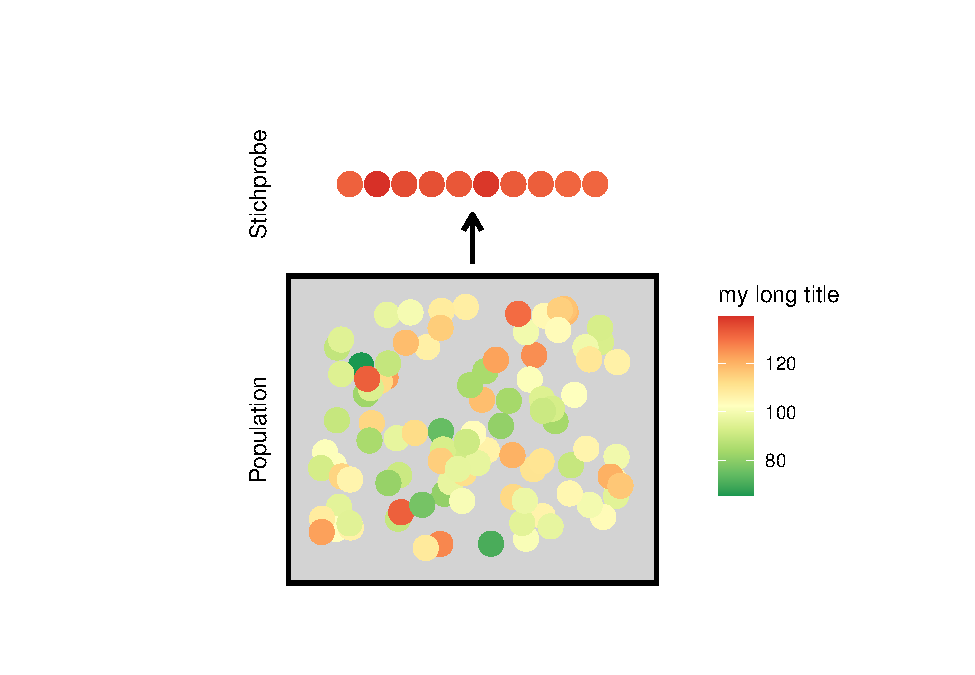
\includegraphics{aps_statistik1_files/figure-latex/stichprobenziehung_intervall-1.pdf}

\section{Was ist das Problem der Stichprobenziehung?}\label{was-ist-das-problem-der-stichprobenziehung}

\section{Wie kann man Aussagen über die Grundgesamtheit machen?}\label{wie-kann-man-aussagen-uxfcber-die-grundgesamtheit-machen}

\section{Übungen}\label{uxfcbungen-1}

\chapter{Durchschnitt und Standardabweichung schätzen}\label{durchschnitt-und-standardabweichung-schuxe4tzen}

\section{Wo liegt der Durchschnitt der Grundgesamtheit?}\label{wo-liegt-der-durchschnitt-der-grundgesamtheit}

\section{Wo liegt der Durchschnitt der Standardabweichung?}\label{wo-liegt-der-durchschnitt-der-standardabweichung}

\section{Übungen}\label{uxfcbungen-2}

\chapter{Durchschnitt testen}\label{durchschnitt-testen}

\section{Entspricht der Durchschnitt der Grundgesamtheit einem gewissen Wert?}\label{entspricht-der-durchschnitt-der-grundgesamtheit-einem-gewissen-wert}

\section{Weicht der gefundene Durchschnitt stark vom hypothetischen Wert ab?}\label{weicht-der-gefundene-durchschnitt-stark-vom-hypothetischen-wert-ab}

\section{Übungen}\label{uxfcbungen-3}

\part{Gruppenvergleich einer intervallskalierten Variable}\label{part-gruppenvergleich-einer-intervallskalierten-variable}

\chapter{Gruppenvergleich einer intervallskalierten Variable}\label{gruppenvergleich-einer-intervallskalierten-variable}

\section{Zwei Gruppen vergleichen}\label{zwei-gruppen-vergleichen}

\section{Was ist das Problem der Stichprobenziehung?}\label{was-ist-das-problem-der-stichprobenziehung-1}

\section{Wie kann man Aussagen über die Grundgesamtheit machen?}\label{wie-kann-man-aussagen-uxfcber-die-grundgesamtheit-machen-1}

\section{Übungen}\label{uxfcbungen-4}

\chapter{Welch-Test}\label{welch-test}

\section{Zwei Gruppen vergleichen}\label{zwei-gruppen-vergleichen-1}

\section{Sind die Durchschnitte der beiden Gruppen in der Grundgesamtheit gleich?}\label{sind-die-durchschnitte-der-beiden-gruppen-in-der-grundgesamtheit-gleich}

\section{Wie stark unterscheiden sich die Durchschnitte?}\label{wie-stark-unterscheiden-sich-die-durchschnitte}

\section{Übungen}\label{uxfcbungen-5}

  \bibliography{book.bib,packages.bib}

\end{document}
